
% 
% Annual Cognitive Science Conference
% Sample LaTeX Paper -- Proceedings Format
% 

% Original : Ashwin Ram (ashwin@cc.gatech.edu)       04/01/1994
% Modified : Johanna Moore (jmoore@cs.pitt.edu)      03/17/1995
% Modified : David Noelle (noelle@ucsd.edu)          03/15/1996
% Modified : Pat Langley (langley@cs.stanford.edu)   01/26/1997
% Latex2e corrections by Ramin Charles Nakisa        01/28/1997 
% Modified : Tina Eliassi-Rad (eliassi@cs.wisc.edu)  01/31/1998
% Modified : Trisha Yannuzzi (trisha@ircs.upenn.edu) 12/28/1999 (in process)
% Modified : Mary Ellen Foster (M.E.Foster@ed.ac.uk) 12/11/2000
% Modified : Ken Forbus                              01/23/2004
% Modified : Eli M. Silk (esilk@pitt.edu)            05/24/2005
% Modified : Niels Taatgen (taatgen@cmu.edu)         10/24/2006
% Modified : David Noelle (dnoelle@ucmerced.edu)     11/19/2014

%% Change "letterpaper" in the following line to "a4paper" if you must.

\documentclass[10pt,letterpaper]{article}

\usepackage{cogsci}
\usepackage{pslatex}
\usepackage{apacite}
\usepackage{amsmath,amssymb}
\usepackage{graphicx}
\usepackage{color}
\usepackage{url}
%\newcommand{\url}[1]{$#1$}


\definecolor{Red}{RGB}{255,0,0}
\newcommand{\red}[1]{\textcolor{Red}{#1}}

 \newcommand{\denote}[1]{\mbox{ $[\![ #1 ]\!]$}}


\newcommand{\subsubsubsection}[1]{{\em #1}}
\newcommand{\eref}[1]{(\ref{#1})}
\newcommand{\tableref}[1]{Table \ref{#1}}
\newcommand{\figref}[1]{Figure \ref{#1}}
\newcommand{\appref}[1]{Appendix \ref{#1}}
\newcommand{\sectionref}[1]{Section \ref{#1}}

\title{Wonky worlds: Listeners revise world knowledge when utterances are odd}
%\title{Wonky worlds: Listeners reconsider world knowledge when utterances are odd}
%Non-sinking marbles are wonky: defeasible world knowledge in language interpretation}

 
\author{{\large \bf Judith Degen, Michael Henry Tessler, Noah D.~Goodman} \\
  \{jdegen,mhtessler,ngoodman\}@stanford.edu\\
  Department of Psychology, 450 Serra Mall \\
  Stanford, CA 94305 USA}

% ggplot colors: "#F8766D", "#A3A500", "#00BF7D", "#E76BF3", "#00B0F6"

% variations on blue: "#007fb1", "#4ecdff"

\begin{document}

\maketitle


\begin{abstract}
World knowledge enters into pragmatic utterance interpretation in complex ways, and may be defeasible in light of speakers' utterances.  Yet there is to date a surprising lack of systematic investigation into the role of world knowledge in pragmatic inference. In this paper, we show that a state-of-the-art model of pragmatic interpretation greatly overestimates the influence of world knowledge on the interpretation of utterances like \emph{Some of the marbles sank}. We extend the model to capture the idea that  the listener is uncertain about the background knowledge the speaker is bringing to the conversation. This extension greatly improves model predictions of listeners' interpretation and also makes good qualitative predictions about listeners' judgments of how `normal' the world is in light of a speaker's statement. Theoretical and methodological implications are discussed.

%\red{edit}
%World knowledge enters into pragmatic utterance interpretation in complex ways. Sometimes, a speaker's utterance suggests that listeners should disregard their world knowledge, yet current models of pragmatic interpretation either disregard the role of world knowledge or overestimate its role in interpretation. Here we provide an extension to the Rational Speech Act model of scalar implicature that captures whether listeners believe they are in an abnormal--or `wonky'--world after observing a speaker's utterance, in which case they downweight their prior beliefs in the computation of speaker meaning. We show in four experiments that a) listeners have varying prior beliefs about the probability of various objects exhibiting an effect (e.g., marbles sinking), b) these beliefs influence listeners' expectations about how many objects will show the effect after observing an utterance (like \emph{Some of the marbles sank}), c) these beliefs influence scalar implicature strength, and d) listeners' world wonkiness judgments are affected by the surprisal of the observed utterance under their prior beliefs. The extended model is the first quantitative model that accounts for how rational listeners should integrate world knowledge in pragmatic utterance interpretation, and provides a close match to the empirically obtained data.

\textbf{Keywords:} 
scalar implicature; world knowledge; prior beliefs; experimental pragmatics; computational pragmatics
\end{abstract}

How often do you think marbles would sink in water? Probably extremely often, if not always. Now imagine reading \emph{Max threw fifteen marbles in the water. Some of the marbles sank.} Have you begun to reconsider your assumptions? Perhaps you now suspect that these marbles are in fact made of hollow plastic or the water is covered with thick algae? That is, maybe these are not just normal marbles in normal water. Here we explore how prior world knowledge enters into pragmatic utterance interpretation, and when this world knowledge is defeasible: some utterances lead listeners to conclude that the world under discussion is abnormal and has appropriately different prior probabilities. We refer to such an abnormal world  as a \emph{wonky} world.

The Rational Speech Acts framework (RSA)  \cite{frank2012,goodmanstuhlmueller2013}, and related models \cite{franke2011,russell2012}, treat communication as a signaling game \cite{lewis1969} between a speaker and a listener.
The listener reasons by Bayesian inference about what the world is like given that a speaker who produced the utterance is trying to be informative (with respect to a na\"ive listener). 
Variants of these models have successfully captured listeners' quantitative  behavior on a number of pragmatic inference tasks, including ad hoc Quantity implicature \cite{degenfrankejaeger2013}, markedness implicature \cite{bergengoodman2012}, scalar implicature \cite{goodmanstuhlmueller2013}, and non-literal language \cite{kao2014}. 
A defining feature of Bayesian reasoning is that prior beliefs affect inferences that will be drawn. Bayesian models of language interpretation, accordingly, predict that prior beliefs about the world should affect the listener's interpretation of an utterance. 
%These models make clear predictions about how prior beliefs about states of the world should be integrated with listeners' expectations about utterances a speaker is likely to produce to communicate a particular state of the world. 
While this impact of prior knowledge has been noted, and included in models, it hasn't been systematically studied.

Generalizing our opening example, consider \emph{Some of the X sank}, where \emph{X} is a plural noun such as \emph{marbles}, \emph{feathers}, or \emph{balloons}, and \emph{the X} refers to a contextually established group of objects from category X. When the prior probability, $\theta_{X}$, of an X\footnote{We will use `X' interchangeably to refer to both the category and the members of the category.} sinking is not extreme (e.g., a feather sinking), RSA leads to the standard scalar implicature: the posterior probability that all of the X sank, after hearing the utterance, is much lower than its prior probability (i.e., \emph{Some of the feathers sank} yields that not all of them did). This is because a rational speaker would have been expected to produce the more informative \emph{All of the X sank}, had it been true.
As we will show below, RSA makes two strong predictions about the effect of the prior: (1) As $\theta_{X}$ approaches $1$, the interpretation probability that all X sank approaches $1$, that is, the scalar implicature disappears. 
This prediction follows because the extreme prior overwhelms the effect of the utterance.
(2) For moderate to high prior (roughly $0.5{<}\theta_{X}{<}1$) and a large total number of objects (more than about 10), the posterior expectation of the number of X that sank should be approximately the same as the prior expectation---that is, the utterance shouldn't affect the expected number of X that sank. 
This prediction follows from the weak semantics of \emph{some} and the isolated effect of the alternative \emph{all}: because \emph{Some of the X sank} only restricts the interpretation (i.e., the number of marbles that sank) to be greater than zero, and because the scalar implicature resulting from the alternative \emph{All of the X sank} can at most rule out the state in which all of the X sank, the prior will dominate the inference about exactly how many X sank.



However, intuition is at odds with these predictions: as \citeA{geurts2010} has observed, for events with very high prior probability of occurrence (e.g., marbles sinking), observing an utterance such as \emph{Some of the marbles sank} seems to yield strong implicatures; that is, contrary to RSA predictions the subjective probability that all of the marbles sank is intuitively close to 0. 
%The reason for this is presumably that listeners realize that the speaker went to the trouble of producing an utterance that is weaker than what the prior would lead one to believe.
%

In Exp.~1 we collect prior probabilities for a variety of events (e.g., sinking) and categories (e.g., marbles). In Exps.~2a and 2b we collect corresponding posterior interpretations after observing  utterances containing quantifiers. These experimental results confirm the intuition of relatively strong implicature---hence prediction (1) of RSA is incorrect---and show that the prior has a muted effect on posterior expectation---hence prediction (2) of RSA is incorrect.
Given the previous success of RSA models, this constitutes a striking puzzle. 
To address this puzzle we pursue the intuition raised at the very beginning of this paper: that sometimes, the speaker's utterance will lead the listener to infer that the world under discussion is wonky and she should therefore use less extreme prior beliefs in the computation of speaker meaning. We introduce a variant of RSA, \emph{wonky RSA (wRSA)}, in which the listener can revise her beliefs about the domain under discussion. We show that this extension resolves the puzzle of the prior's muted effects.
In Exp.~3 we explore participants' intuitions about whether the world is normal or wonky in the scenarios of Exps.~2a and 2b and find that wRSA predicts listeners' wonkiness judgements.


\section{Experiment 1: prior elicitation} 

Exp.~1 measured listeners' prior beliefs about how many objects exhibit a certain effect (e.g., how many marbles sink).%, $P(s)$.

\subsection{Method}

\subsubsection{Participants}
We recruited 60 participants over Amazon's crowd-sourcing platform Mechanical Turk.

\subsubsection{Procedure and materials}

On each trial,\footnote{This experiment can be viewed at \url{https://www.stanford.edu/~jdegen/12_sinking-marbles-prior15/sinking-marbles-prior.html}} participants read a one-sentence description of an event like \emph{John threw 15 marbles into a pool.} They were then asked to provide a judgment of an effect, e.g.~\emph{How many of the marbles do you think sank?}, on a sliding scale from 0 to 15. Each item had a similar form: the first sentence introduced the objects at issue (e.g., marbles). The question always had the form \emph{How many of the X Yed?}, where \emph{X} was the head of the direct object noun phrase introduced in the first sentence (e.g., \emph{marbles}, \emph{cups}, \emph{balloons}) and \emph{Yed} was a verb phrase denoting an effect that the objects underwent (e.g., \emph{sank}, \emph{broke}, \emph{stuck to the wall}). Each verb phrase occurred with three different objects, e.g., \emph{sank} occurred with \emph{marbles}, \emph{cups}, and \emph{balloons}. Items were constructed to intuitively cover the range of probabilities as much as possible, while also somewhat oversampling the upper range of probabilities to have more fine-grained coverage of this region that is of most interest for testing the RSA model. Judgments were obtained for 90 items, of which each participant saw a random selection of 30 items. 
%\red{should be more specific about the materials... each item had a similar form, with action, category, and outcome differing? say that we constructed them to cover the range of probabilities as much as possible.}

\subsection{Results}

Data from one participant, who gave only one response throughout the experiment, were excluded. Each item received between 12 and 29 ratings. Distributions of ratings for each item were smoothed using nonparametric density estimation for ordinal categorical variables \cite{liracine2003} with the \verb|np| package in R \cite{hayfield2008}. As intended, items covered a wide range of probabilities. See \figref{fig:probhist} for a histogram of expected values of each smoothed prior distribution.

\begin{figure}
	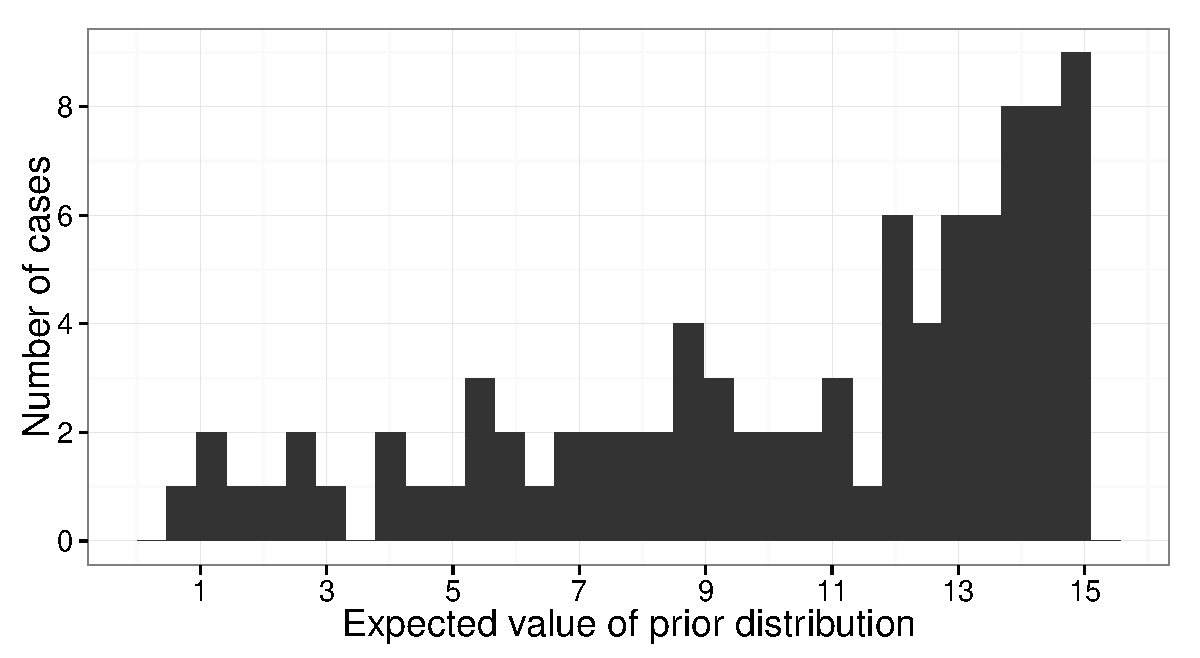
\includegraphics[width=.5\textwidth]{pics/priorexpectations-histogram}	
	\caption{Histogram of expected values of each empirically elicited and smoothed prior distribution.}
	\label{fig:probhist}	
\end{figure}

In the next section, we use these empirically obtained smoothed prior beliefs to derive RSA predictions for the interpretation of utterances like \emph{Some of the marbles sank}, before empirically measuring participants' interpretations.

%\red{say that we succeed in getting items that cover the probability range -- also maybe indicate how close the distributions are to binomial?}



% -illustrate why \emph{some} is weird for high prior.
%-tie in to common ground (or wait for discussion?)

 

%\red{it's bold to make the intro so short.... i feel like a bit more is needed to set the stage for the paper. or possible the next section should just not be a separate section. at any rate, saying early the high level puzzle will help: Bayesian pragmatics sensitivity to the prior, we don't find this sensitivity. We suggest that this is because the (common ground) prior can be revised to accommodate otherwise unexplainable utterances.}




%World knowledge enters into the interpretation of utterances in complex ways. %For example, the plausibility of an NP as the subject of a sentence influences whether listeners are garden-pathed in cases like \textit{The horse raced past the barn fell} vs.~\textit{The landline buried in the sand exploded} \cite{bla}.
%While effects of world knowledge on syntactic processing are well-established, there is to date a surprising lack of systematic investigations into the effect of world knowledge in pragmatics. % -- this is especially surprising given that it has long been noted in the linguistics literature that pragmatics requires the integration of many different sources of linguistic and non-linguistic information. 
%Here, we provide a quantitative model of the effect of world knowledge  on  scalar implicatures, which are inferences that arise in cases of utterances like \textit{Some of the marbles sank}, %like (\ref{marbles}), where an utterance of (\ref{somemarbles}) 
%which typically gives rise to the inference that not all of the marbles sank.% in (\ref{simarbles}).
%
%\begin{exe}
%	\ex\label{marbles} 
%	\begin{xlist}
%		\ex\label{somemarbles} Some of the marbles sank.
%		\ex\label{simarbles} Not all of the marbles sank.
%	\end{xlist}
%\end{exe}


\section{Effect of the world prior in RSA}

The basic Rational Speech Acts model defines a pragmatic listener $P_{L_1}(s|u)$, who reasons about a speaker $P_{S_1}(u|s)$, who in turn reasons about a literal listener $P_{L_0}(s|u)$. Each listener does Bayesian inference about the world state, given either the literal truth of utterance $u$ or the speaker's choice of $u$; the speaker is a softmax-optimal decision maker, with the goal of being informative about the state $s$.
RSA is defined by:
\begin{eqnarray}
&&P_{L_0}(s|u)\propto \delta_{\denote{u}(s)} \cdot P(s)\\
&&P_{S_1}(u|s) \propto \mathrm{exp}({\lambda \ln P_{L_0}(s|u))}\\ 
&&P_{L_1}(s|u)\propto P_{S_1}(u|s)\cdot P(s)
\end{eqnarray}
Here $\denote{u}: S \rightarrow \text{Boolean}$ is a truth-function specifying the literal meaning of each utterance.

For concreteness, assume that the set of states of the world is $S = \{s_0, s_1, s_2, \dots, s_{15}\}$, where the subscript indicates the number of objects (e.g., marbles) that exhibit an effect (e.g., sinking). 
Further assume that the set of utterances \emph{All/None/Some of the marbles sank} is denoted $U = \{u_{\textrm{all}}, u_{\textrm{none}}, u_{\textrm{some}}\}$ and each has its usual literal meaning: 
%$\denote{u_{\textrm{none}}}: s=0$,  
%$\denote{u_{\textrm{some}}}: s>0$,
%$\denote{u_{\textrm{all}}}: s=15$.
$\denote{u_{\textrm{none}}}= \{s_i | i = 0\}$,  
$\denote{u_{\textrm{some}}}= \{s_i | i > 0\}$,
$\denote{u_{\textrm{all}}}= \{s_i | i = 15\}$.

%Let us imagine that the prior is binomial with single event probability $\theta$: $P(s)=\text{Binomial}(s|\theta)$.

\begin{figure*}
	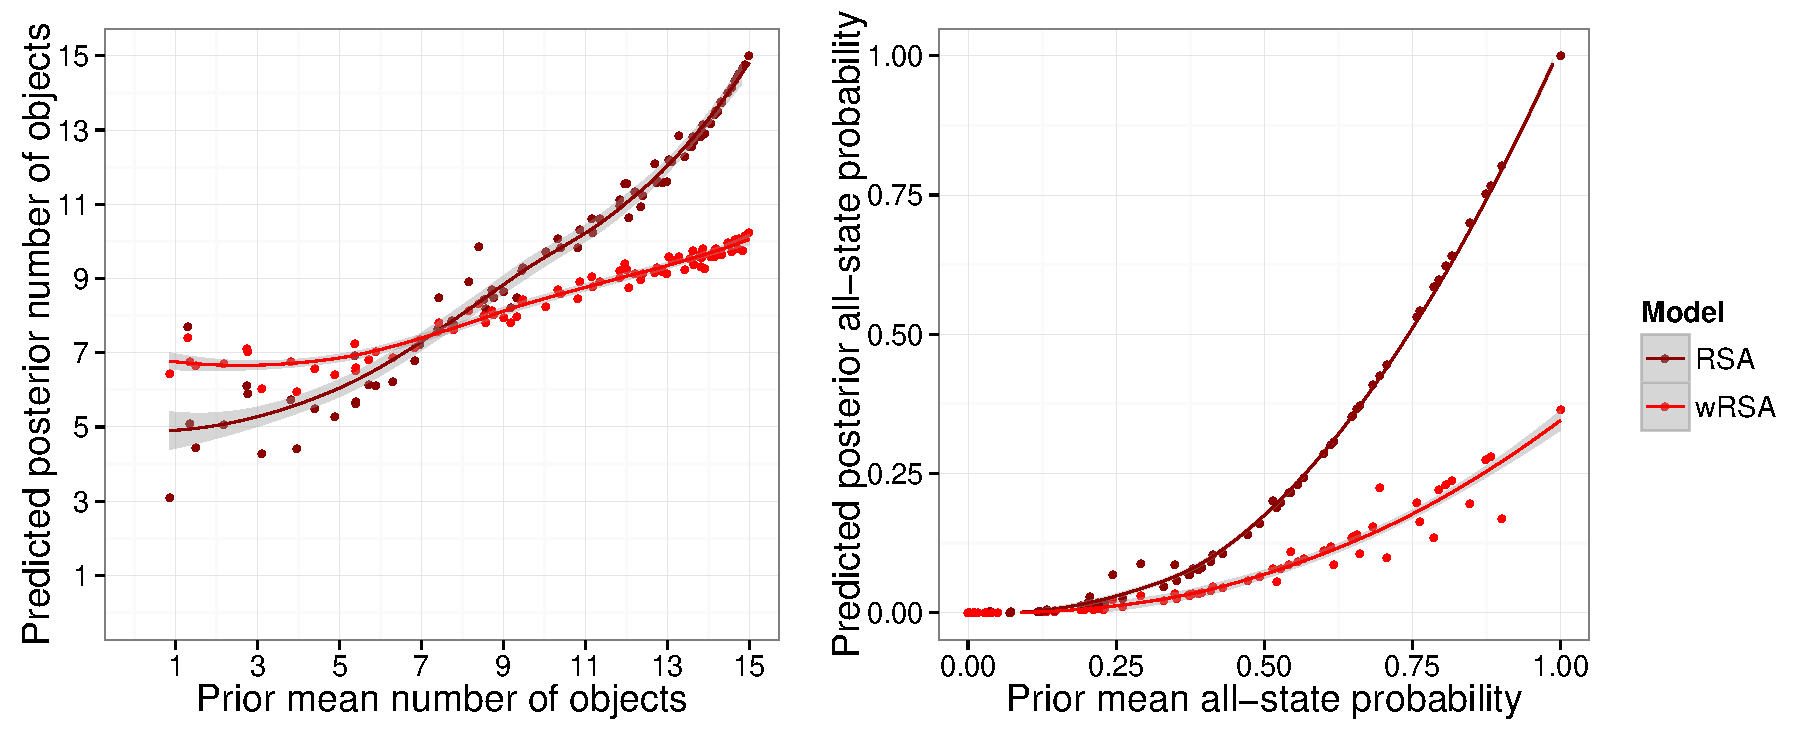
\includegraphics[width=\textwidth]{pics/rsa-predictions}
%	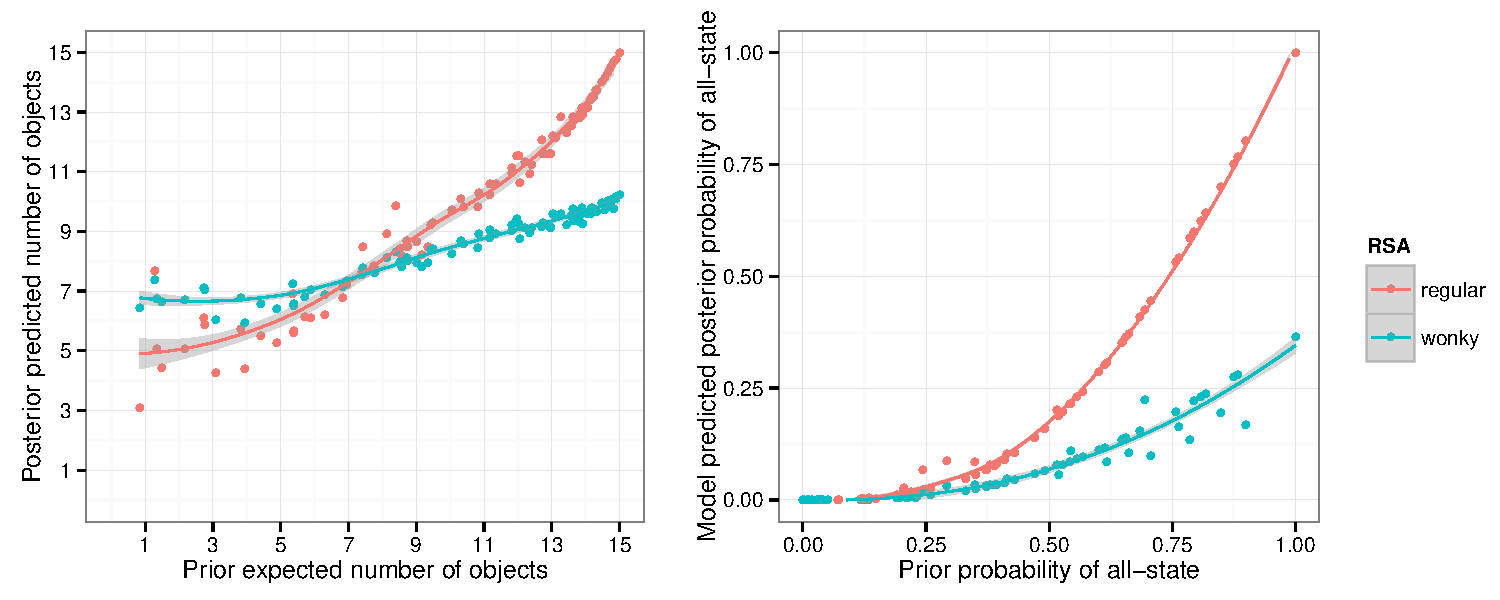
\includegraphics[width=\textwidth]{pics/rsa-predictions-uniform}	
	\caption{For each item, RSA and wRSA model predicted $\mathbb{E}[P(s|u_{\textrm{some}})]$ as a function of $\mathbb{E}[P(s)]$ (left) and $P(s_{15}|u_{\textrm{some}})$ as a function of $P(s_{15})$ (right).}
	\label{fig:rrsaexppredictions}	
\end{figure*}

In Figure \ref{fig:rrsaexppredictions} we show the predictions of RSA (dark blue dots) for the items from Exp.~1 in two different ways: the left panel shows the posterior expected number of affected objects as a function of the prior expectation; the right panel shows the posterior probability of the state in which all objects are affected, as a function of the prior probability of that state.\footnote{That the individual model predictions look somewhat noisy is due to the different shapes of the prior distributions, such that for the same expected value of the distribution, the distribution itself can take different shapes, which will be treated slightly differently by the model.}   %as $\theta$ varies. \red{put in figure showing the basic RSA predictions for allstate $P(s_{15}|u_{some})$ and expectation. this figure could also have wRSA predictions for later reference.} 
We see that the prior has a strong effect, which can be summarized by the two predictions described in the Introduction: 
(1) $P(s_{15}|u_{\textrm{some}}) \rightarrow 1$ as $P(s_{15})\rightarrow 1$. 
(2) $\mathbb{E}[P(s|u_{\textrm{some}})] \simeq \mathbb{E}[P(s)]$ over the upper half of its range. 
We next turn to an empirical test of these predictions, or rather, of the intuition that they may be incorrect.

%\section{Models of utterance interpretation}
%
%
%Recent Bayesian Rational Speech Act (RSA)  \cite{frank2012} and game-theoretic \cite{franke2011} models that treat communication as a signaling game \cite{lewis} between a speaker and a listener have successfully captured listeners' quantitative  behavior on a number of pragmatic inference tasks, including ad hoc Quantity implicature \red{ref}, M-implicature \red{ref}, scalar implicature \red{ref}, and embedded scalar implicatures \red{ref}. In these models, the listener reasons about likely utterances a speaker will produce who is trying to be informative with respect to a na\"ive listener. These models make clear predictions about how prior beliefs about states of the world should be integrated with listeners' expectations about utterances a speaker is likely to produce to communicate a particular state of the world. 
%
%\red{i think we should hold the math for the model section. it doesn't really add much here... without it, this section can be folded nicely into the introduction.}
%
%For concreteness, assume that $S = \{s_0, s_1, s_2, \dots, s_{15}\}$ is the set of states of the world, where the subscript indicates the number of objects (e.g., marbles) that exhibit a certain effect (e.g., sinking). Assume further that $U = \{u_{\textrm{all}}, u_{\textrm{none}}, u_{\textrm{some}}\}$, the set of utterances \emph{All/None/Some of the marbles sank}. The speaker chooses an utterance to convey $s$ proportional to the soft-max expected utility of producing $u$ to communicate $s$, where utility is determined by how uncertain a listener remains: \red{what's the expectation doing?}
%
%\begin{equation}
%P_{S_1}(u|s) \propto \mathrm{exp}({\lambda \mathbb{E} (\ln P_{\textrm{lex}}(s|u))})
%\end{equation}
%
%where $P_{\textrm{lex}}(s|u)$ is the literal interpretation probability resulting from each utterance's truth-functional meaning: $F_u: s \mapsto \{0,1\}$. \red{need to spell out lit listener since the prior enters there too} The listener's task is to infer a distribution over $S$, given an utterance $u$ produced by the above defined informative speaker. %$p(s|u)$, that is, the probability of the state of the world the speaker intended to communicate (e.g., how many friends came to a party), given that the speaker produced $u$ (e.g., \emph{some of my friends came to the party}). 
%By Bayes' rule: 
%\begin{equation}
%P_{L_1}(s|u)\propto P_{S_1}(u|s)\cdot P(s)
%\end{equation}
%That is, the inferred listener probabilities are proportional to the product of both the speaker's utterance probabilities and the listener's prior beliefs in different numbers of marbles sinking. Using a uniform prior over the state space, this model has been very successful at capturing \emph{scalar implicatures} \cite{grice1975}. These are inferences that arise in cases of utterances like \textit{Some of the marbles sank}, which typically give rise to the inference that not all of the marbles sank. Scalar implicatures fall out of the fact that the speaker probability of producing $u_{\textrm{some}}$ in $s_{15}$ is low (because there is an alternative utterance $u_{\textrm{all}}$ which has a higher probability of being used for $s_{15}$ because it is more informative about that state). However, the role of prior beliefs in RSA models remains under-explored, both with respect to scalar implicature computation as well as with respect to utterance interpretation more generally.
%
%
%%One important consequence of the standard RSA model is that the listener's prior beliefs will not affect the interpretation of $u$ very strongly, if at all,  where the semantics of $u$ is highly constraining, that is, where  $P_{\textrm{lex}}(s|u)$ is very peaked. For example, an utterance of \emph{All of the marbles sank} is highly constraining because all of the probability mass ends up on $s_{15}$ by virtue of the semantics of $u_{\textrm{all}}$ alone, regardless of how likely the listener believes marbles sink a priori.\footnote{We ignore hyperbolic interpretations of universal quantifiers here.} 
%
%One important consequence of the standard RSA model is that where the semantics of $u$ is weak---that is, where $F_u$ accepts many states---prior beliefs are predicted to have a large effect on the resulting listener belief distribution. For example, an utterance of \emph{Some of the marbles sank}, produced in a situation in which any of 0 - 15 of 15 contextually established marbles could have sunk, semantically only restricts the state space by one state (that in which 0 marbles sank). In this case, listeners' prior beliefs about sinking marbles will have a large effect on their posterior belief distribution. If the listener believes that marbles rarely sink, the utterance will be interpreted as conveying that fewer marbles sank than if the listener believes marbles almost always sink. The predictions this model makes for the interpretation of $u_{\textrm{some}}$ -- both for $P_{L_1}(s_{15}|u_{\textrm{some}})$ and for the expected value of $P_{L_1}(s|u_{\textrm{some}})$ as a function of $P(s_{15})$ and the expected value of $P(s)$, respectively  -- are shown in \figref{fig:rrsaexppredictions}. RSA predicts that the probability of the state in which all objects exhibit a certain effect increases with increasing $P(s_{15})$, such that for $P(s_{15})$ close to 1, $P_{L_1}(s_{15}|u_{\textrm{some}})$ approaches 1. Relatedly, with increasing expected value of the prior belief distribution $P(s)$, so is the expected value of the posterior belief distribution predicted to increase, approaching 1). \red{hmm... i think we either need to focus on the allstate probs for this motivation, or already point to the data from expt 1.}
%
%However, intuition is at odds with this prediction: for example,  \citeA{geurts2010} has observed that for events with very high prior probability of occurrence (e.g.~marbles sinking), observing an utterance of \emph{Some of the marbles sank} leads to very strong implicatures, that is, the subjective probability  that not all of the marbles sank is intuitively close to 0. Given the previous success of RSA models, this constitutes a striking puzzle, and one we set out to solve here. In doing so, we pursue the intuition raised at the very beginning of this paper: that sometimes, the speaker's utterance will lead the listener to infer that the world under discussion is wonky and she should therefore down-weight her prior beliefs in the computation of speaker meaning.
%
%
%Our contribution is two-fold: first, we collect empirical estimates of $P(s)$ and $P_{L_1}(s|u)$ to investigate the empirical effect of listeners' prior beliefs on interpretation. Second, we extend the RSA model to incorporate a free variable $\theta_{\textrm{wonky}}$ that captures the extent to which the listener believes the described event is wonky  and she should thus discount her prior beliefs when interpreting $u$. We refer to this model as \emph{wonky RSA (wRSA)} in contrast to \emph{regular RSA (rRSA)}. Wonkiness inferences in wRSA are triggered by the surprisal of a produced utterance $u$, given listeners' prior beliefs, capturing that listeners expect speakers' utterances to be both truthful and informative with respect to prior beliefs. To the extent that they are not, listeners will have to either infer that the speaker is being uncooperative, or else assume that they may need to revise their beliefs about the world. Here we pursue the latter possibility.
%
%This paper is structured as follows. We first report the results of three experiments (1, 2a, 2b) that show that while there is an effect of the prior on listeners' interpretations of sentences like \emph{Some of the marbles sank}, this effect is much smaller than predicted by rRSA. Exp.~3 provides evidence that listeners' beliefs about object or event wonkiness are indeed influenced by the surprisal of the utterance. Finally, we present wRSA as an extension of rRSA that incorporates the idea of backing off to alternate prior beliefs if the observed utterance suggests a wonky world. This model provides a much better fit to the empirical data from Exps.~2a and 2b than rRSA, and also provides a good fit to the wonkiness ratings obtained in Exp.~3.




\section{Experiment 2a and 2b: comprehension}  
%\red{if we end up tight on space, the expt 2a and 2b sections can be combined.}

%\red{i think the current 2b should go first, since it uses the same DM as expt 1....}

Exps.~2a and 2b\footnote{These experiments can be viewed at \url{https://www.stanford.edu/~jdegen/13_sinking-marbles-priordv-15/sinking-marbles.html} and \url{https://web.stanford.edu/~jdegen/16_sinking-marbles-sliders-certain/sinking-marbles-nullutterance.html}}  measured participants' posterior beliefs $P(s|u)$ about how many objects exhibited a certain effect (e.g., marbles sinking), after observing an utterance. The only difference between the experiments was the dependent measure. The dependent measures differed in order to directly and independently estimate the two values that the  predictions above are concerned with: $\mathbb{E}[P(s|u_{\textrm{some}})]$ and $P(s_{15}|u_{\textrm{some}})$.

\subsection{Method}

\subsubsection{Participants}
For each experiment we recruited 120 participants over Amazon's Mechanical Turk.

\subsubsection{Procedure and materials}

Participants read the same descriptions as in Exp.~1. They additionally saw an utterance produced by a knowledgeable speaker about the event, e.g.~\textit{John, who observed what happened, said: ``Some of the marbles sank''}. In Exp.~2a (just as in Exp.~1), they then provided a judgment of an effect, e.g.~\textit{How many of the marbles do you think sank?}, on a sliding scale from 0 to 15. In Exp.~2b they instead rated on sliding scales with endpoints labeled ``definitely not'' and ``definitely'', how likely they thought 0\%, 1-50\%, 51-99\%, or 100\% of the objects exhibited the effect.

Each participant saw 10 \emph{some} trials and 20 filler trials, of which 10 contained the quantifiers \emph{all} or \emph{none}, and the rest were utterances that did not address the number of objects that displayed the effect. Of these, half were generic short fillers that were intended to communicate the prior, e.g., \emph{Typical}. The rest were longer sentences that addressed a different aspect of the described scenario, e.g.~\emph{What a stupid thing to do}. The utterances were randomly paired with 30 random items for each participant.

 
\begin{figure*}
	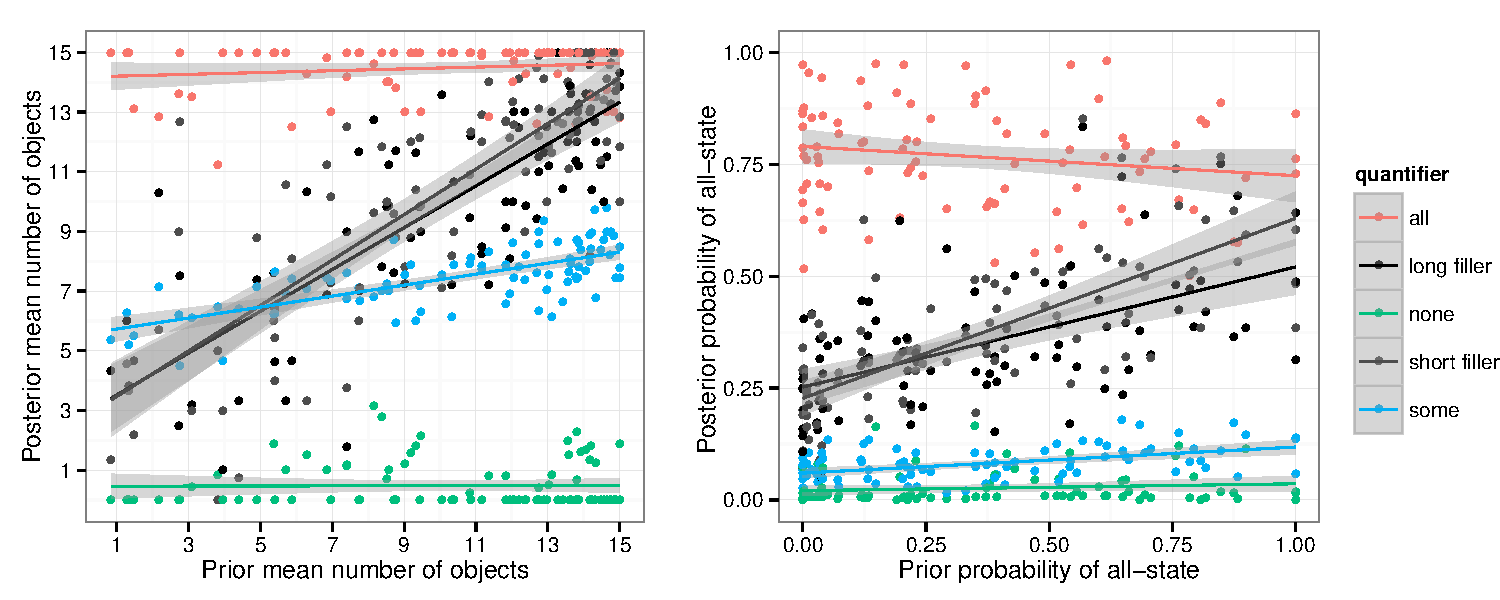
\includegraphics[width=\textwidth]{pics/empirical-results}	
	\caption{For each item and quantifier, (left) empirical $\mathbb{E}[P(s|u_{\textrm{some}})]$ vs. $\mathbb{E}[P(s)]$, that is Exp.~2a vs.~Exp.~1,  and (right) empirical $P(s_{15}|u_{\textrm{some}})$ vs.~$P(s_{15})$, that is Exp.~2b vs.~Exp.~1.}
	\label{fig:empiricalresults}	
\end{figure*}

 
 \subsection{Results and discussion}

Data from eight participants in Exp.~2b were excluded from the analysis because these participants assigned less than .8 probability to the interpretation corresponding to the correct literal interpretation on literal \emph{all} and \emph{none} trials. 

The main question of interest was whether participants' judgments of how many objects exhibited the effect after hearing an utterance with \emph{some} followed the predictions of the basic RSA model laid out in the previous section. Mean empirical $\mathbb{E}[P(s|u)]$ and $P(s_{15}|u)$ are shown in \figref{fig:empiricalresults} for each item. There was a small effect of the prior. For utterances of \emph{Some of the X Yed}, the mean number of objects judged to exhibit the effect increased with increasing expectation of the prior distribution ($\beta$=.18, $SE$=.02, $t$=7.4, $p$$<$.0001). Similarly, the probability of all 15 objects exhibiting the effect increased with increasing prior probability of doing so ($\beta$=.06, $SE$=.01, $t$=5.0, $p$$<$.0001). However, the size of these effects is astronomically smaller than predicted by RSA (for comparison, see dark lines in \figref{fig:rrsaexppredictions}).% that is, \citeA{geurts2010}'s observation that implicatures are very strong even for very likely events is confirmed empirically.

One possible explanation for this highly attenuated effect of the prior is that participants simply do not bring world knowledge to bear on the interpretation of utterances. However, this possibility is ruled out by examining participants' performance in the filler conditions: in both Exps.~2a and 2b, the filer conditions closely tracked the prior (see \figref{fig:empiricalresults}). 

Exps.~2a and 2b demonstrate that there is an effect of listeners' prior beliefs on the interpretation of utterances with \emph{some}. However, this effect is quantitatively much smaller than predicted by RSA, and qualitatively does not match the predictions identified above: the implicature is not canceled for extreme priors and the posterior expectation diverges from the prior expectation.
In the next section, we extend the RSA model to formalize a listener who may decide that her initial beliefs about the domain are not shared by the speaker and responds by revising her priors.


\section{Effect of the world prior in `wonky RSA'}

To capture the idea that the pragmatic listener is unsure what background knowledge the speaker is bringing to the conversation, we extend the basic RSA model by using a ``lifted variable'' \cite{goodmanlassiter,lassiter2013,bergengoodman2012,kao2014} corresponding to the choice of state prior. That is, we posit that the prior, now $P(s|w)$, depends on a ``wonkiness'' variable $w$, which determines if it is the ``usual'' prior for this domain or a more generic back-off prior that we take to be uniform:
$$
P(s|w) \propto \begin{cases}
1  & \text{if } w\\
   P_{\text{usual}}(s) & \text{if not } w
  \end{cases}
  $$
  
This inferred prior is used in both the literal and pragmatic listeners, indicating that it is taken to be common ground. However, the $w$ variable is reasoned about only by the pragmatic listener, which captures the idea that it is an inference the pragmatic listener makes about which assumptions are appropriate to the conversation. Using the notation of the earlier modeling section:
\begin{eqnarray}
&&P_{L_0}(s|u,w)\propto \denote{u}(s) \cdot P(s|w)\\
&&P_{S_1}(u|s,w) \propto \mathrm{exp}({\lambda \ln P_{L_0}(s|u,w))}\\
&&P_{L_1}(s,w|u)\propto P_{S_1}(u|s,w)\cdot P(s|w) \cdot P(w)
\end{eqnarray}
We refer to this model as wRSA. Notice that the choice of $w$ that the listener makes will depend on $P_{S_1}(u|s,w)$: if a given utterance can't be explained by the usual prior, because it is unlikely under any plausible world state $s$, then the pragmatic listener will infer that the world is wonky, and back off to the uniform prior.
That is, if the utterance is odd, the listener will revise her opinion about what world knowledge is appropriate to use.

To make predictions for Exp.~2 from wRSA we use the smoothed empirical priors from Exp.~1 as $P_{\text{usual}}(s)$ for each item. The wonkiness prior $P(w)$ and the speaker optimality $\lambda$ are fit to optimize mean squared error (MSE) with Exp.~2 data. The optimal parameters ($\lambda = 2$, $P(w) = 0.5$) resulted in an MSE of 2.15 (compared to 14.53 for RSA) for the expected number of objects, and 0.01 (compared to 0.07 for RSA) for the all-state probability. The better fit of wRSA compared to RSA can be seen in the comparison of \figref{fig:rrsaexppredictions} and \figref{fig:empiricalresults}: in both cases, wRSA (light blue lines) predicts a much attenuated effect of the prior compared to regular RSA (dark blue lines), in line with the empirical data. Furthermore, wRSA does not make either of the problematic predictions identified earlier for regular RSA.


These results are encouraging: wRSA is able to account for the qualitative and quantitative departures of participants' behavior from RSA, with respect to the effect of the prior.
Is this because listeners are actually inferring that the world is unusual from an utterance like \emph{Some of the marbles sank}?
The wRSA model makes predictions about the probability that a given world is wonky after observing an utterance; see \figref{fig:wonkymodel} for predicted wonkiness probabilities for $u_{\textrm{all}}$, $u_{\textrm{none}}$, and $u_{\textrm{some}}$ using the  optimal $P(w)$ and $\lambda$ parameters from fitting wRSA to the Exp.~2 data.
Note the U-shaped curve, in which the world is judged wonky if $u_{\textrm{some}}$ is used in worlds with extreme priors.
 We can test these predictions directly by simply asking participants whether the situation is normal.



\begin{figure}
%	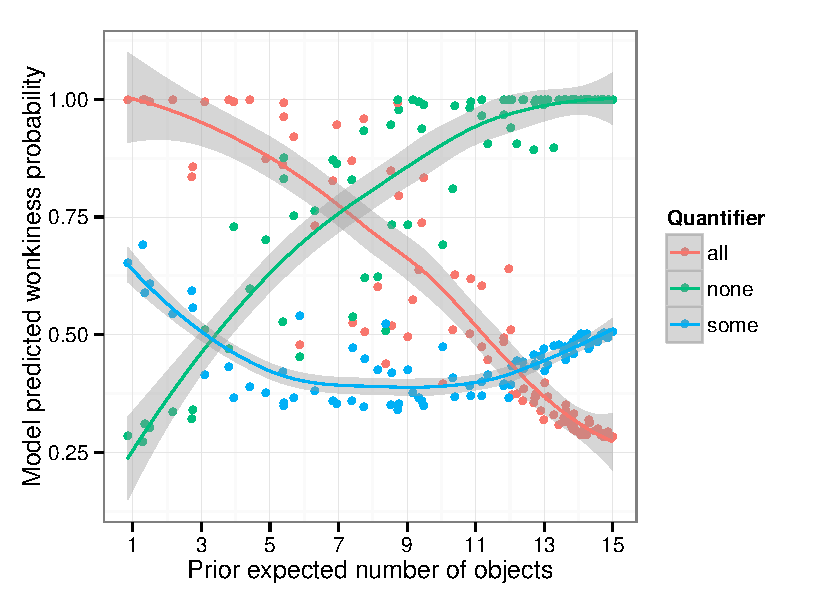
\includegraphics[width=.5\textwidth]{pics/model-wonkiness-binomial}
	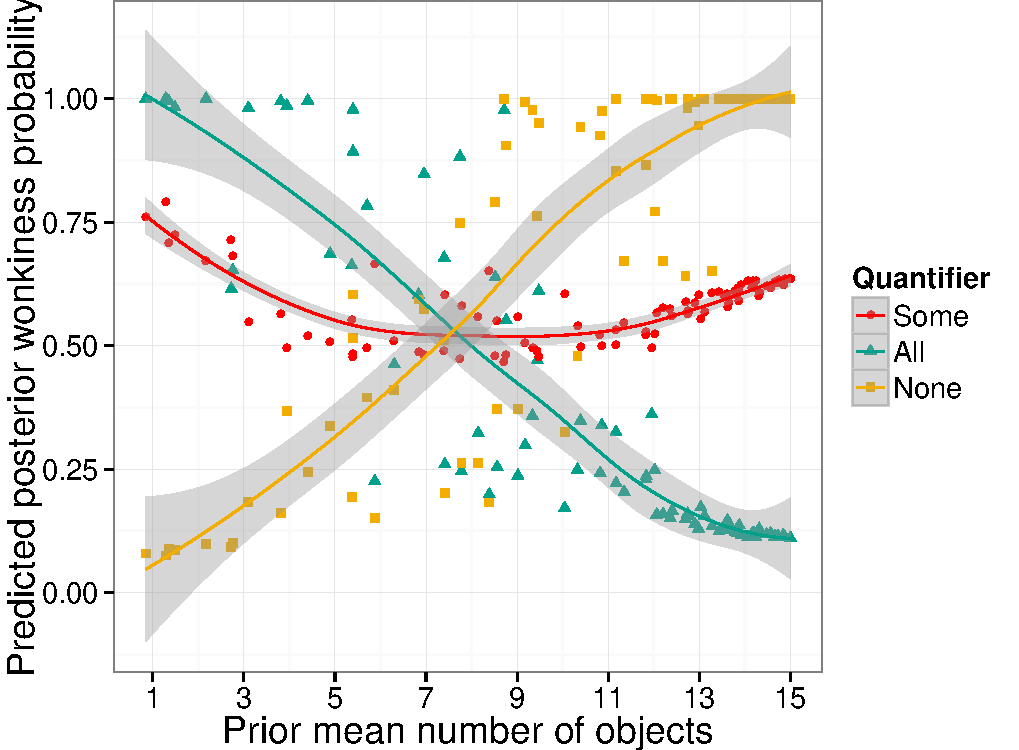
\includegraphics[width=.5\textwidth]{pics/model-wonkiness-uniform}
	\caption{For each item, predicted wonkiness probability after observing an utterance ($u_{\textrm{all}}, u_{\textrm{none}}, u_{\textrm{some}}$), as a function of the prior expected number of affected objects.}
	\label{fig:wonkymodel}	
\end{figure}

\section{Experiment 3: wonkiness}

Exp.~3\footnote{This experiment can be viewed at \url{https://web.stanford.edu/~jdegen/17_sinking-marbles-normal-sliders/sinking-marbles-normal.html}} measured participants' beliefs in world wonkiness after observing the scenarios and utterances from Exps.~2a and 2b.

\subsubsection{Participants}
We recruited 60 participants over Amazon's crowd-sourcing platform Mechanical Turk.

\subsubsection{Procedure and materials}

The procedure and materials were identical to those of Exps.~2a and 2b, with the exception of the dependent measure. Rather than providing estimates of what they believed the world was like, participants were asked to indicate how likely it was that the objects  (e.g., the marbles) involved in the scenario were normal objects, by adjusting a slider that ranged from \emph{definitely not normal} to \emph{definitely normal}.

\subsubsection{Results}

The extreme ends of the sliders were coded as 1 (\emph{definitely not normal}, i.e., wonky) and 0 (\emph{definitely normal}, i.e., not wonky). We interpret the slider values as probability of world wonkiness. Mean wonkiness probability ratings are shown in \figref{fig:wonkyratings} and closely mimic wRSA's predictions (see \figref{fig:wonkymodel}). For $u_{\textrm{all}}$ and $u_{\textrm{none}}$, increasing prior expectation of objects exhibiting the effect resulted in a fairly linear decrease and increase in the probability of wonkiness, respectively. For $u_{\textrm{some}}$, the pattern is somewhat more intricate: probability of wonkiness initially decreases sharply, but rises again in the upper range of the prior expected value. 

\begin{figure}
	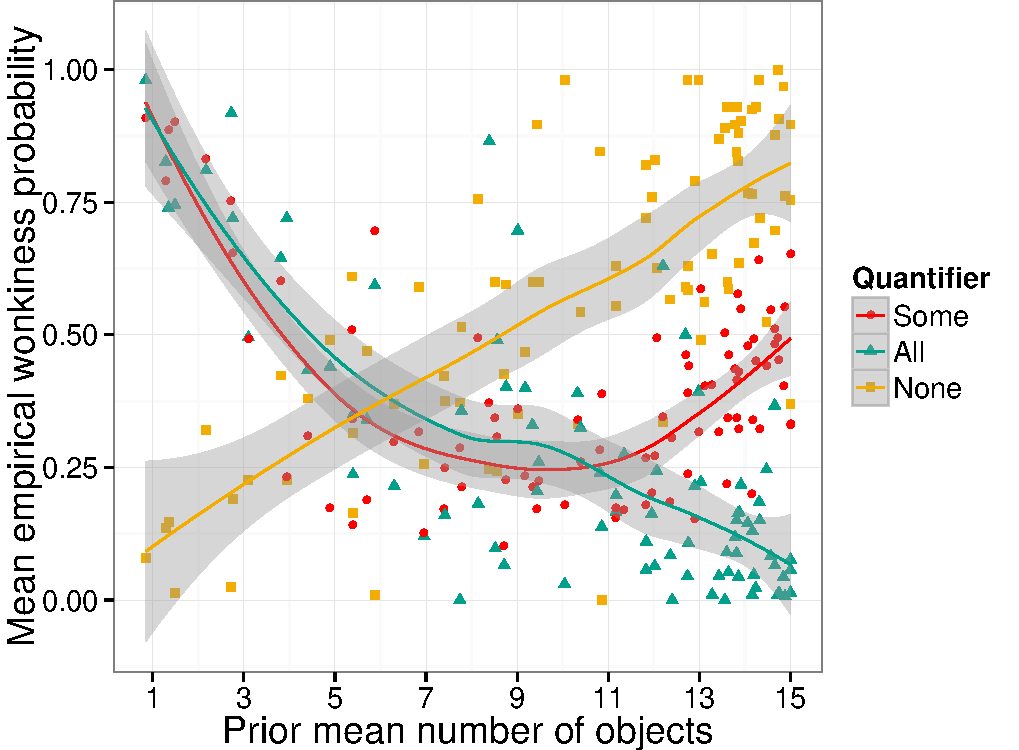
\includegraphics[width=.5\textwidth]{pics/empirical-wonkiness}
	\caption{For each item, mean empirical wonkiness probability after observing an utterance ($u_{\textrm{all}}, u_{\textrm{none}}, u_{\textrm{some}}$), as a function of the prior expected  number of affected objects.}
	\label{fig:wonkyratings}	
\end{figure}

Qualitatively, the model captures both the linear increase and decrease in wonkiness probability for $u_{\textrm{all}}$ and $u_{\textrm{none}}$, respectively. Importantly, it also captures the asymmetric U-shaped wonkiness probability curve displayed by $u_{\textrm{some}}$. Intuitively, this shape can be explained as follows: for very low probability events, it is surprising to learn that such an event took place (which is what is communicated by $u_{\textrm{some}}$), so wonkiness is high. For medium probability events, learning that this event took place is not very surprising, so wonkiness is relatively low. For high probability events, $u_{\textrm{some}}$ may be literally true, but it would not be useful in the sense of providing the listener new information. For comparison to the comprehension data fit, the model's MSE for empirical wonkiness probability predictions, using the best parameters from fitting the model to the comprehension data, was 0.07. 




%This `lifted variable' that can be conceived of as analogous to the lifted variable over lexica that is at the core of recent lexical uncertainty models of word learning \red{ref}, M-implicature, and embedded scalar implicature \cite{bergen2014}. The difference is that, rather than having uncertainty about the lexicon the listener believes the speaker to be employing, the listener has uncertainty about the speaker's prior beliefs. In particular, the speaker uses either the empirical prior (obtained in Exp.~1) or an alternative prior \red{DESCRIBE}. The pragmatic listener 


%\red{it's possible we'd get less noise form some more stable estimator of prior. consider trying the plots with prior mode and median as x-axis.... or inferred binomial prob fit to each prior, if the fits are at all decent.}



%\red{NDG: note to self -- difference between revising own beliefs and revising common ground....}


\section{Discussion and conclusion}


%% discussion and conclusions
% - "This suggests that in certain situations, listeners update their prior beliefs in the computation of speaker meaning." --> "listeners revise their prior beliefs...".... updating priors seems like Bayesness as usual.. technically, we're updating our prior on priors, no?



%Interlocutors bring a wealth of world knowledge to bear on any language interpretation task. While effects of world knowledge in different areas of language processing are well-established (\red{psycholinguistics refs}), there has to date been a surprising lack of quantitative investigation into the role of world knowledge--and its defeasibility--in pragmatic inference. 
We have shown that listeners' world knowledge, in the form of prior beliefs, enters into the computation of speaker meaning in a systematic but subtle way. The effect of the prior on interpretation was much smaller, and qualitatively different, than predicted by a standard Bayesian model of quantifier interpretation (RSA). 
This suggests that in certain situations, listeners revise their assumptions about relevant priors as part of the computation of speaker meaning. 
Indeed, in the cases where the largest deviations from RSA obtained, participants also judged the world to be unusual.
%We have provided empirical evidence that the types of situations that lead to such revision , that is, situations in which the speaker's utterance is too unlikely given the listener's default prior beliefs and the available utterance alternatives. are cases of `wonky' worlds
Extending RSA with a lifted wonkiness variable that captures precisely whether listeners think the world is unusual, and allows them to back off to a uniform prior (i.e., ignore entirely their previously held beliefs about the world), provided a good fit to the empirical wonkiness judgements and dramatically improved the fit to participants' comprehension data. This model constitutes the first attempt to explicitly model the quantitative effect of world knowledge and its defeasibility on pragmatic utterance interpretation and raises many interesting questions.

In one sense the revision of beliefs in the wRSA listener is standard Bayesian belief updating with respect to a complex prior; however it is not the simple belief update of a flat or hierarchical prior, because the different aspects of prior belief (i.e.~$P(w)$ and $P(s|w)$) interact in complex ways with the listener's assumptions about the speaker.
As a result, an odd utterance can lead the listener to update their own view of $w$; this in turn impacts both their own prior over states and what prior they believe the speaker believes they are using---an odd utterance leads the listener to re-evaluate common ground. 
This is reminiscent of linguistic theories of presupposition accommodation \cite{lewis1979,stalnaker1973,stalnaker1998}.
It will be interesting to further explore the relation of the wRSA approach to presupposition.

Throughout this paper we discussed wonkiness as an attribute of the \emph{world}, yet empirically we elicited wonkiness judgments about the \emph{objects} involved in the events. 
This raises the question of what exactly listeners are revising about their prior beliefs: objects, events, the speaker's beliefs, or the way the speaker uses language? 
%Relatedly, in the current implementation of wRSA, prior belief revision has a global effect: that is, the prior that the listener infers is simultaneously the prior the listener attributes to the speaker; that is, the prior is treated as being in common ground, and the revision of the prior thus leads to a revision of common ground. But it is in fact an empirical question whether listeners revise their own privileged beliefs about the world, their beliefs about the common ground, or their beliefs about the speaker's beliefs. \red{WONKY SENTENCE: Addressing this question in future research will reveal whether a more complex mechanism for prior belief revision needs to incorporated that explicitly models prior vs.~privileged ground.}
Relatedly, we have used a uniform prior distribution as the alternative to consider when the listener believes the world is wonky.  One could imagine various more flexible alternatives. For instance, listeners may make minimal adjustments to their prior knowledge, or alternatively, may prefer extreme priors that rationalize the utterance once they have discounted the usual priors.
%Do metaphorical interpretations draw listeners out of the wonky world? 
Future research should investigate the options listeners have available when their world knowledge must be revised to accommodate an utterance.

This work also has methodological implications: researchers working in the field of experimental semantics and pragmatics would be well served to take into account the effect of `odd' items, prior beliefs, and interactions between the two.\footnote{For an in depth discussion of this issue in syntactic processing, see, e.g., \citeA{jaeger2010, fine2013a}.} In particular, if the attempt to design uniform stimuli across conditions yields odd utterances in some conditions, we predict that participants will respond by revising their prior beliefs in ways that can be unpredictable. That is, we expect unpredictable interaction effects between stimuli and conditions. This is likely to inflate or compress potential effects of an experimental manipulation. 

Concluding, this work exemplifies the importance and utility of exploring the detailed quantitative predictions of formal models of language understanding.
Exploring the prior knowledge effects predicted by RSA led us to understand better the influence of world knowledge and its defeasibility on pragmatic interpretation.
Listeners have many resources open to them when confronted with an odd utterance, and re-construing the situation %, rather than giving up the assumption of speaker cooperativity, 
appears to be a favorite.


%\begin{itemize}
%
%%	\item what is wonky? -- objects, event, speaker? -- connection to adaptation?
%%	\item other ways of asking about wonkiness
%%	\item \red{what's the right prior to back off to?}
%%	\item revising private beliefs vs revising common ground.
%%	\item \red{connection to presupposition (cf stalnaker), and other phenomena}
%%	\item implication for experiments on language understanding
%
%\end{itemize}



\bibliographystyle{apacite}

\setlength{\bibleftmargin}{.125in}
\setlength{\bibindent}{-\bibleftmargin}

\bibliography{bibs}


\end{document}
